\clearpage{\pagestyle{empty}\cleardoublepage}
\chapter{Caratteristiche della memoria cache}

\begin{flushright}\begin{small}\textit{"The beginning of knowledge\\
 is the discovery of something we do not understand."}\\
- Frank Herbert -\\
\end{small}\end{flushright}

Si \`e scelto di progettare una cache di tipo set-associative, la cui schematizzazione \`e mostrata in Fig. \ref{fig:set_ass}.
Questa tipologia di cache rappresenta un buon compromesso tra flessibilit\`a e costo in termini di silicio.

\begin{figure}[!h]
\centering
% \includegraphics[scale=0.8]{img/set-associative.jpg}
\includegraphics[width=\textwidth]{img/set-associative.jpg}
\caption{Schematizzazione di una cache set-associative}
\label{fig:set_ass}
\end{figure}


L'indirizzo di partenza del blocco \`e diviso in TAG (parte alta), INDEX e OFFSET (parte bassa).
Il TAG consente di identificare univocamente una linea all'interno di un un sottoinsieme di linee, detto SET.
L'INDEX individua immediatamente il SET all'interno del quale \`e possibile recupeare la linea corrente tramite il confronto del TAG.
In questo modo si limita il numero di confronti tra TAG accettando il fatto che ogni linea possa appartenere ad un singolo set.
%Ogni linea pu\`o essere memorizzata in una qualsiasi delle vie dello slot individuato dall'INDEX.
La parte meno significativa dell'indirizzo rappresenta l'OFFSET che consente di individuare il dato all'interno di una linea.

Per garantire maggiore flessibilit\`a si \`e scelto di parametrizzare alcune delle caratteristiche statiche della cache,

quali ad esempio:
\begin{itemize}
\item la dimensione dei blocchi
\item il numero di vie
\item il numero di linee
\end{itemize}


\section{Politica di rimpiazzamento}

Nel caso in cui si debba caricare una nuova linea e tutte le vie siano occupate \`e necessario determinare quale linea rimpiazzare.
Un buon algoritmo di rimpiazzamento dovrebbe cercare di individuare la linea "vittima" che meno probabilmente verr\`a riutilizzata in seguito.
Il criterio scelto per effettuare il rimpiazzamento \`e basato su contatori, che implementa una politica LRU (Least Recently Used).
Tale politica \`e tipicamente implementata poich\`e statisticamente si verifica principio di localit\`a.
\`E quindi presente un contatore per ogni via di ogni set tramite il quale si tiene traccia di quanto recentemente si \`e acceduti a ciascuna linea: un valore basso del contatore indica un accesso recente mentre un valore alto indica un accesso\emph{vetusto}.
Evidentemente la linea candidata al rimpiazzamento risulta essere quella alla quale \`e associato il contatore di valore pi\`u elevato.
Nel caso di HIT su una linea, sono incrementati i valori di contatori pi\`u basso rispetto al valore di quello della linea HIT mentre quest'ultimo viene resettato.
Nel caso di MISS si procede con un rimpiazzamento e poi si agisce come nel caso di HIT sulla nuova linea.
Infine, in caso di invalidazione di una linea, si porta al valore massimo il contatore della linea invalidata e si decrementano di 1 tutti i contatori con valore pi\`u elevato di quello della linea invalidata.


\section{Struttura e interfacce}
La memoria cache si interfaccia con i dispositivi esterni attraverso 3 tipi di interfacce, come mostrato in Fig. \ref{fig:int_gen}.

\begin{figure}[!h]
 \centering
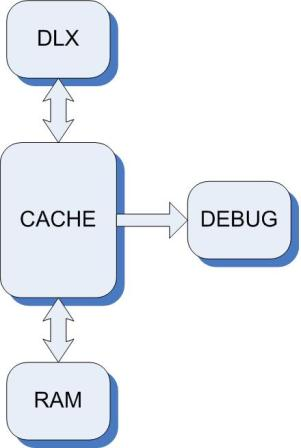
\includegraphics{img/01-interfacce_schema_generale.jpg}
 \caption{Interfacce della memoria cache}
 \label{fig:int_gen}
\end{figure}


L'interfaccia verso il micropocessore, mostrata in Fig. \ref{fig:int_dlx}, consente a quest'ultimo di accedere ai dati memorizzati all'interno della cache. 

\begin{figure}[!h]
 \centering
\includegraphics{img/dlx-cache.jpg}
 \caption{Interfaccia della memoria cache verso il processore DLX}
 \label{fig:int_dlx}
\end{figure}

In particolare sono presenti i seguenti segnali:
\begin{itemize} %i nomi dei comandi non sono esatti: vanno sostituiti
\item \textbf{Address[31-2]}: indirizzi a 32 bit emessi dal microprocessore
\item \textbf{Data[32-0]}: bus dati con parallelismo 32bit 
\item \textbf{Write}: segnale per il comando di scrittura in cache
\item \textbf{Read}: segnale per il comando di lettura da cache
\item \textbf{Ready}: segnale che indica il termine dell'operazione di lettura/scrittura corrente
\end{itemize}

L'interfaccia verso la RAM, mostrata in Fig. %\ref{fig:int_ram}
, consente alla cache di recuperare i blocchi dal livello sottostante.

%\begin{figure}[!h]
% \centering
%\includegraphics{img/ram-cache.jpg}
% \caption{Interfaccia della memoria cache verso la RAM}
% \label{fig:int_dlx}
%\end{figure}

In particolare sono presenti i seguenti segnali:
\begin{itemize} %i nomi dei comandi non sono esatti: vanno sostituiti
\item \textbf{Address[31-2]}: indirizzi a 32 bit emessi dalla cache
\item \textbf{Data[32-0]}: bus dati con parallelismo 32bit 
\item \textbf{Write}: segnale per il comando di scrittura in RAM
\item \textbf{Read}: segnale per il comando di lettura dalla RAM
\item \textbf{Ready}: segnale che indica il termine dell'operazione di lettura/scrittura corrente
\end{itemize}

Si noti che la cache non \`e a conoscenza del componente posto al livello superiore. Vista la simmetria delle due interfacce \`e quindi possibile sostituire la RAM con un ulteriore livello di cache. inserendo quindi pi\`u livelli di cache all'interno del processore.\\
\`E presente infine una terza interfaccia verso l'esterno, utilizzata per monitorare lo stato interno della cache e poter quindi eseguire il debug.
I segnali disponibili verranno definiti nel seguito.\\
Si ipotizza che la memoria cache progettata non sia impiegata in sistemi multimaster. Per tale motivo non si considereranno problematiche inerenti alla presenza di un controllore di memoria e all'invalidazione delle linee.










